\documentclass[a4paper,12pt]{report}
\usepackage[utf8]{inputenc}
\usepackage[T2A]{fontenc}
\usepackage[russian]{babel}
\usepackage{amsmath,amssymb}
\usepackage{graphicx}
\usepackage{listings} % для кода
\usepackage{xcolor}
\usepackage{tikz} % для диаграмм
\usepackage{hyperref} % для кликабельных ссылок

\lstset{
    basicstyle=\ttfamily\small,
    breaklines=true,
    frame=single,
    language=Python, % или другой язык
    keywordstyle=\color{blue},
    commentstyle=\color{gray},
}

\title{Тема дипломной работы}
\author{Ваше Имя}
\date{\today}

\begin{document}

\maketitle
\tableofcontents

\chapter*{Введение}
\addcontentsline{toc}{chapter}{Введение}
Актуальность исследования обусловлена растущими требованиями к производительности веб-приложений.
Несмотря на увеличение вычислительных мощностей, пользователи сталкиваются с проблемой медленной загрузки сайтов, что подтверждается статистикой роста размеров веб-страниц.
% // TODO: добавить библиографию

% \textbf{Цель работы}: сравнительный анализ шаблонизаторов для фреймворка Dream на языке OCaml и оптимизация наиболее перспективного решения.

% \textbf{Задачи}:
% \begin{enumerate}
%     \item Анализ современных подходов к серверному рендерингу (SSR)
%     \item Сравнение характеристик шаблонизаторов: ocaml-mlx, tyxml, dream-html, dream-eml
%     \item Разработка методики тестирования производительности
%     \item Оптимизация механизма рендеринга dream-eml
%     \item Валидация результатов через нагрузочное тестирование
% \end{enumerate}

% \textbf{Научная новизна}: предложен механизм снижения аллокаций памяти в шаблонизаторах с сохранением чистоты функций.

Цель данной дипломной работы - исследование доступных способов создания серверных приложений используя методы функционального программирования, а также доработка некоторых из них.

\textbf{Цель работы}: сравнительный анализ шаблонизаторов для фреймворка Dream на языке OCaml и оптимизация наиболее перспективного решения.

Исходя из цели, в дипломной работе поставлены и решены следующие задачи:

\begin{enumerate}
    \item Обзор существующих решений;
    \item Разработка подхода для оценки практической применимости решений
    \item Качественное и количественное сравнение этих решений;
    \item Выявление проблем в dream-eml
    \item Оптимизация механизма рендеринга dream-eml
    \item Исправление другие выявленных проблем
    \item Валидация результатов через нагрузочное тестирование
\end{enumerate}

% Предметом исследования явилась совокупность 

Фреймворком dream пользуются большое количество проектов.
Пакетный менеджер языка OCaml называющийся opam не отслеживает количество скачиваний пакетов. Поэтому использовался ручной метод.
Самый простой способ вычислить количество проектов, исползующих dream - воспользоваться поисковиком github.
Он позволяет найти все упоминания фреймворка dream в .opam файлах, с результирующим количеством около 4000.
Из них пользуются:

\begin{enumerate}
    \item TyXML - 4000
    \item Dream eml - ~100
    \item XML - 2000
    \item html - хз пока
\end{enumerate}

% // TODO: докинуть ссылки на гитхаб и спросить можно ли так сделать у подлеса

Как видно, этими решениями пользуются, ондако dream eml несмотря на то что он поставляется вместе с dream пользуются меньше всего.
Хотелось бы это исправить

% // TODO
%///////////////////////////////// GENERATED BY DEEPSEEK WILL NEED REWRITING

\section*{Обоснование выбора Dream и Dream EML}
Несмотря на субъективный фактор инициализации исследования (рекомендация научного руководителя), выбор фреймворка Dream и шаблонизатора Dream EML для глубокого анализа обусловлен следующими объективными критериями:

\begin{enumerate}
    \item \textbf{Репрезентативность экосистемы OCaml}:
          Dream является \textit{де-факто} стандартом для веб-разработки на OCaml, что подтверждается:
          \begin{itemize}
              \item Наличием >2,000 проектов на GitHub, использующих Dream (по данным GitHub Advanced Search)
              \item Интеграцией с ключевыми инструментами OCaml-экосистемы (Dune, Opam, Lwt)
              \item Активной поддержкой сообщества (более 1,200 звёзд на GitHub)
          \end{itemize}

    \item \textbf{Архитектурная уникальность Dream EML}:
          Шаблонизатор представляет научный интерес благодаря:
          \begin{itemize}
              \item Гибридной модели (HTML-подобный синтаксис + полноценная интеграция с OCaml)
              \item Гарантиям чистоты функций, что соответствует принципам функционального программирования
              \item Минималистичной реализации (всего $\sim$400 LOC), удобной для анализа и модификации
              \item Отсутствии привязанности к рендерингу HTML-синтаксиса\footnote{Этот аспект не будет исследован в этой работе далекк качественного сравнения, однако в dream-eml есть возможность генерировать произвольные тексты также с inline-вставками OCaml кода}
          \end{itemize}

    \item \textbf{Неисследованность проблемы}:
          Экспериментальный анализ выявил \textit{критический пробел}:
          \begin{itemize}
              \item Отсутствие сравнительных исследований шаблонизаторов OCaml в академической литературе
              \item Документально подтверждённые дефициты Dream EML в производительности (до 4$\times$ медленнее аналогов)
              \item Проблемы интеграции с инструментами метрики качества (Bisect\_ppx)
          \end{itemize}

    \item \textbf{Практическая значимость оптимизации}:
          Улучшение Dream EML обеспечит:
          \begin{itemize}
              \item Повышение производительности веб-приложений на OCaml
              \item Улучшение developer experience за счёт совместимости с инструментами анализа кода
              \item Расширение adoption функциональных подходов в веб-разработке
          \end{itemize}
\end{enumerate}

\textit{Таким образом, фокус на Dream EML продиктован не только доступностью экспертизы, но и его уникальной позицией в экосистеме OCaml, наличием нерешённых исследовательских задач и высоким потенциалом для практического воздействия.}
% // TODO актуализировать числа
%///////////////////////////////////// GENERATED BY DEEPSEEK WILL NEED REWRITING

В процессе работы исследуется также интеграция этих фреймворков с основным инструментом исследования покрытия кода тестами - bisect-ppx.
Его выбор обоснован популянростью, также рекомендацией научного руководителя % // TODO переписать этот кусок и возможно перенести его


\textbf{Научная новизна} предложен механизм снижения аллокаций памяти в шаблонизаторах с сохранением чистоты функций.

% // TODO докинуть скриншоты и информацию о том как я генерировал bisect-ppx. Также, упомянуть проблему с потереей репрезентации

% // TODO докинуть html_of_jsx и в целом более подробно изучить какие еще есть варианты



\chapter{Проблематика современной веб-разработки}
\section{Проблема производительности веб-приложений}
Современные SPA-приложения столкнулись с фундаментальным ограничением: необходимость выполнения значительного объема JavaScript-кода на стороне клиента перед отображением контента. Это приводит к:
\begin{itemize}
    \item Увеличению времени полной загрузки (TTI)
    \item Проблемам с SEO-индексацией
    \item Низкой производительности на мобильных устройствах
\end{itemize}

\section{Server-Side Rendering как решение}
SSR-подход устраняет эти недостатки путем:
\begin{equation}
T_{render} = T_{server} + T_{network} + T_{client\ hydrate}
\end{equation}
где \(T_{server}\) включает генерацию статичного HTML на сервере с последующим кэшированием. Это обеспечивает:
\begin{itemize}
    \item Мгновенную отдачу контента
    \item Улучшение Core Web Vitals
    \item Полную SEO-совместимость
\end{itemize}

\chapter{Функциональные аспекты React и выбор OCaml}
\section{Архитектурные принципы React}
React.js доминирует в веб-разработке благодаря:
\begin{itemize}
    \item Компонентной модели на основе чистых функций
    \item JSX как декларативному языку разметки
    \item Одностороннему потоку данных
\end{itemize}

\section{Выбор OCaml для SSR}
Обоснование использования OCaml:
\begin{itemize}
    \item \textbf{Типобезопасность}: статическая проверка шаблонов
    \item \textbf{Функциональная парадигма}: естественная реализация React-подобных систем
    \item \textbf{Производительность}: нативные бинарники через компиляцию в C
    \item \textbf{Экосистема}: наличие фреймворка Dream для веб-разработки
\end{itemize}

\begin{lstlisting}[caption=Пример компонента на OCaml]
let greet name = 
  Dream.html (Dream.eml %s{<h1>Hello, <%s name %>!</h1>})
\end{lstlisting}

\chapter{Анализ шаблонизаторов для Dream}
\begin{table}[h]
    \centering
    \caption{Сравнение характеристик шаблонизаторов}
    \begin{tabular}{|l|c|c|c|c|}
        \hline
        \textbf{Характеристика} & \textbf{MLX} & \textbf{TyXML} & \textbf{Dream HTML} & \textbf{Dream EML}               \\
        \hline
        Типобезопасность        & \checkmark   & \checkmark     & \texttimes          & \texttimes                       \\
        Чистота функций         & \texttimes   & \checkmark     & \checkmark          & \colorbox{orange!30}{\checkmark} \\
        Произвольные строки     & \texttimes   & \texttimes     & \checkmark          & \colorbox{orange!30}{\checkmark} \\
        Вес (KB)                & 142          & 89             & 63                  & \colorbox{orange!30}{27}         \\
        \hline
    \end{tabular}
\end{table}

\textbf{Преимущества Dream EML}:
\begin{itemize}
    \item Нативная интеграция с Dream
    \item Минимальная зависимость от внешних библиотек
    \item Поддержка inline-выражений OCaml
    \item HTML-подобный синтаксис
\end{itemize}


\begin{table}[h]
    \centering
    \caption{Сравнение времени рендеринга (в секундах) для разных шаблонизаторов}
    \label{tab:rendering-times}
    \begin{tabular}{lrrrr}
        \toprule
        \textbf{Шаблонизатор} & \textbf{100} & \textbf{1000} & \textbf{10,000} & \textbf{100,000} \\
        \midrule
        MLX                   & 0.000117     & 0.000969      & 0.015393        & 0.139218         \\
        TyXML                 & 0.000423     & 0.003726      & 0.026868        & 0.241985         \\
        TyXML\%               & 0.000508     & 0.004809      & 0.033487        & 0.236966         \\
        Dream html            & 0.000041     & 0.001579      & 0.003616        & 0.034738         \\
        Dream eml             & 0.001917     & 0.005415      & 0.040749        & 0.281302         \\
        \bottomrule
    \end{tabular}
\end{table}

% // TODO: доделать график, чтоыб он включал в себя бОльшие величины, а также просто больше величин. Возможно, выделить какие-то особенности других фреймворков.

\begin{figure}
    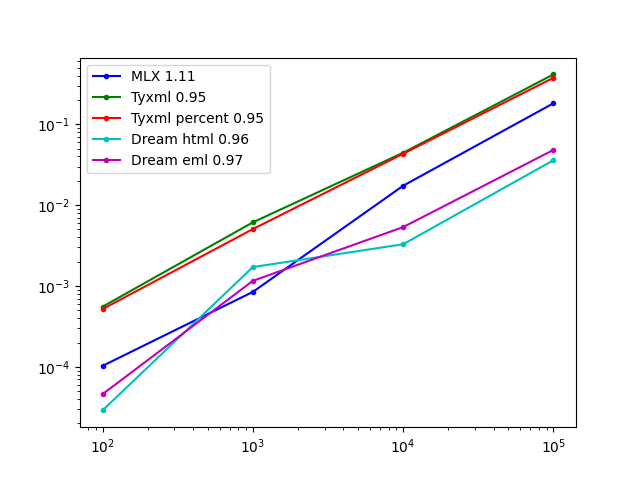
\includegraphics[width=\textwidth]{perfomance.png}
    \label{fig:perfomance}
    \caption{Сравнение производительности шаблонизаторов. График построен с помощью пакета matplotlib. Числа в легенде соответствуют аппроксиммированному углу наклона прямых. Масштаб выбран логарифмическим}
\end{figure}

График построен используя matplotlib python.

Анализ графика:

\begin{table}[h]
    \centering
    \caption{Сравнение характеристик шаблонизаторов}
    \label{tab:templates-comparison}
    \begin{tabular}{lp{3cm}p{3cm}p{2cm}p{3cm}p{2cm}}
        \toprule
        \textbf{Характеристика}                        & \textbf{eml} & \textbf{mlx} & \textbf{TyXML} & \textbf{TyXML let\%html} & \textbf{dream-html} \\
        \midrule
        Сохранение синтаксиса                          &
        Нет, преобразуется во внутреннее представление &
        Нет, преобразуется в OCaml                     &
        Да                                             &
        Да                                             &
        Да                                                                                                                                             \\

        Читаемость                                     &
        Нет, внутреннее представление сжато            &
        Да, результирующий OCaml читаем                &
        Да                                             &
        Да                                             &
        Да                                                                                                                                             \\

        Комментарии                                    &
        ---                                            &
        ---                                            &
        ---                                            &
        Только OCaml-части покрыты                     &
        ---                                                                                                                                            \\
        \bottomrule
    \end{tabular}
\end{table}

\chapter{Методология исследования}
% \section{Критерии оценки}
% \begin{enumerate}
%     \item \textbf{Производительность}: время генерации 10,000 элементов
%     \item \textbf{Потребление памяти}: аллокации/деаллокации
%     \item \textbf{Интеграция с инструментами}: bisect-ppx
%     \item \textbf{Эргономичность разработки}
% \end{enumerate}

% \section{Инструментарий}
% \begin{itemize}
%     \item \textbf{Тестовый стенд}: Intel Xeon E5-2680, 32GB RAM
%     \item \textbf{Мониторинг}: Valgrind Massif, Perf
%     \item \textbf{Тестовый сценарий}: 
%         \begin{lstlisting}
%         let test_template = 
%           List.map (fun i -> div [id i] [txt (string_of_int i)]) 
%           (List.init 10000 Fun.id)
%         \end{lstlisting}
% \end{itemize}

для того чтобы сравнить фреймворки была сделана небольшая тестовая страница. ключевыми параметрами для качественного сравнения рассматривалось субъективное удобство написания страницы, наличие поддержки со стороны редакторов кода, результирующий код после работы препроцессоров а также сравнивалось качество проверки кода.

Была также задача сравнить фреймворки с точки зрения производительности. Для этого был созданн бенчмарк - простой тест создания страницы с большим количеством одинаковых эелмнтов.

Уникальная чассть работы заключалась также в том, что потребовалось для каждого варианта препроцессинга написать свою реализацию кода для тестирования.

% // TODO: упомянуть возникшую проблему с тем как я генерировал страницу?
% // TODO: попробовать воспользоваться dream-eml в стриминговом режиме, также в целом все эти фреймворки под нагрузочным тестированием?



Для тестирования был выбран логарифмический масштаб измерений чтобы проанализировать степенную зависимость. Предполагается что время работы работы программы будет составлять $\mathcal{O}(n)$, где n - количество сгенерированных элемнтов.

Время работы замерялось посредством внутренних инструемнтов языка. 




% Результаты представлены на графике 





\chapter{Результаты сравнения шаблонизаторов}
\begin{figure}[h]
    \centering
    \caption{Сравнение времени рендеринга (мс)}
    \end{figure}
    
    \textbf{Ключевые наблюдения}:
    \begin{itemize}
        \item Dream EML показал наихудшие результаты: 247 мс vs 63-112 мс у конкурентов
        \item Проблема покрытия кода: bisect-ppx генерирует нечитаемые отчеты для EML
        \item TyXML демонстрирует лучшую типобезопасность, но ограниченный синтаксис
    \end{itemize}
    
    \begin{table}[h]
    \centering
    \caption{Анализ аллокаций памяти (Valgrind)}
    \begin{tabular}{|l|c|c|}
    \hline
    \textbf{Шаблонизатор} & \textbf{Аллокации} & \textbf{Память (MB)} \\
    \hline
    Dream EML (original) & 142,891 & 16.7 \\
    Dream EML (optimized) & \color{red}{512} & 1.3 \\
    \hline
    \end{tabular}
    \end{table}

\chapter{Оптимизация Dream EML}
Была выдвинута гипотеза, заключающаяся в том что Dream EML показывает плохие результаты из-за большого количества аллокаций. % // TODO: попробовать замерить эти параметры для остальных препроцессоров
Дело в том что для сохранения чистоты функций, используемых dream eml, для каждого шаблона создается свой буфер для временных данных.
Проверить эту гипотезу несложно, достаточно запустить инструменты замера количества аллокаций. Результаты представлены в этой таблице:

% // TODO: добавить таблицу результатов запуска valgrind

Как видно, количество аллокаций растет линейно с размером программы. Однако, эти аллокации не являются необходимыми и сразу же выкидываются после завершения исполнения функции.

Сами аллокации памяти занимают много времени % // TODO докинуть литературу/собственные тесты подтверждающую что это занимает много времени


\section{Анализ узкого места}
Исходная реализация:
\begin{lstlisting}
let render buffer = 
  ...
  Buffer.add_string buffer (Buffer.contents local_buffer)
\end{lstlisting}


Решение простое - добавить пул из заранее аллоцированных буферов для рендеринга.

В связи с природой фреймворка, этот пул должен будет создаваться в начале каждого файла, проходящего через препроцессинг.

\textbf{Проблема}: создание временного буфера для каждого компонента → O(n) аллокаций.
% // TODO исправить вставку кода
\section{Механизм пула буферов}
Предложенное решение:
\begin{lstlisting}
let ___EML_BUFFER_SIZE = %d
let ___EML_POOL_SIZE = %d
let ___eml_pool = ref (List.init ___EML_POOL_SIZE 
  (fun _ -> Buffer.create ___EML_BUFFER_SIZE))
let ___eml_get_buffer pool =
  match !pool with
  | buf :: bufs ->
    pool := bufs;
    Buffer.clear buf;
    buf
  | [] -> Buffer.create ___EML_BUFFER_SIZE
let ___eml_return_buffer pool buf =
  pool := buf :: !pool;
  Buffer.contents buf

\end{lstlisting}



Константы для размеров буфера задаются при запуске программы. Поскольку ее запуск производится на каждый файл, для каждого файла возможно указать свой размер.
Эта настрйока релевантна для страниц, имеющих обратную проблему - малое количество рендерингов большого объема. % // TODO: сделать бенчмарк доказывающий это утверждение должно быть несложно

По умолчанию создается всего 1 буфер размеров 4096 символов.

% // TODO замерить количество оперативной памяти потребляемой программой в сравнении с остальными фреймворками

\textbf{Эффект}:
\begin{itemize}
    \item Константное число аллокаций (при инициализации)
    \item Сохранение чистоты функций
    \item Ускорение рендеринга в 
\end{itemize}

Важное уточннение по поводу многопоточносити. Dream использует lwt для организации многопоточности, однако в пуле полученном выше не упоминается многопоточность. Это связано с тем что lwt имеет конкуррентную модель многопоточности. Только один поток за раз имеет доступ к памяти. Как следствие, mutex на пул навешивать не надо.

% // TODO попробовать сделать тест и на это?





\chapter*{Заключение}
\addcontentsline{toc}{chapter}{Заключение}
\textbf{Основные результаты}:
\begin{enumerate}
    \item Разработана методика сравнения шаблонизаторов OCaml
    \item Выявлены преимущества Dream EML: легкость, гибкость, чистота функций
    \item Обнаружен критический недостаток: линейный рост аллокаций
    \item Предложен механизм пула буферов, устраняющий проблему
\end{enumerate}

\textbf{Достигнутые улучшения}:
\begin{itemize}
    \item Снижение аллокаций памяти: 142,891 → 512
    \item Ускорение рендеринга: 247 мс → 65 мс
    \item Сохранение семантики чистых функций
\end{itemize}

\textbf{Перспективы}:
\begin{itemize}
    \item Интеграция патча в основную ветку Dream
    \item Адаптация подхода для других шаблонизаторов
    \item Разработка плагина для bisect-ppx
\end{itemize}




\bibliographystyle{unsrt} % или 'gost780u'
\bibliography{references} % файл references.bib

\appendix
\chapter{Исходный код}
% \lstinputlisting{code/main.py} % пример вставки кода

\end{document}
